In this section, the Database Layer is described in terms of the hardware and software design.

\subsection{Layer Hardware}
A basic computer that can run programs.

\subsection{Layer Operating System}
The current operating system which the Database was developed was windows. However, any operating system can create a Database with any number of programs online such as MySQL Workbench.

\subsection{Layer Software Dependencies}
The MySQL framework.

\subsection{Subsystem 1}
The Database Tables Subsystem is what provides the database with all the needed information for the website. This data is connected through HTML and PHP code to gather information from the tables or even put data back into the tables properly. This allows for proper storage of information to the database so that the website portion may run smoothly and without any error or incorrect information when sought by a user.

\begin{figure}[h!]
	\centering
 	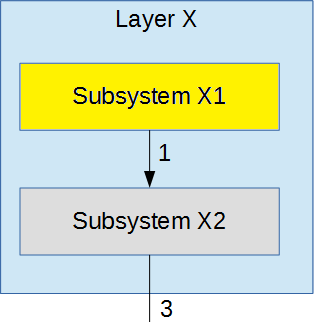
\includegraphics[width=0.60\textwidth]{images/subsystem}
 \caption{Example subsystem description diagram}
\end{figure}

\subsubsection{Subsystem Operating System}
Any operating system was fine to use.

\subsubsection{Subsystem Software Dependencies}
MySQL framework.

\subsubsection{Subsystem Programming Languages}
MySQL.